\section{Applications}

We discuss different types of verification checks enabled by the proposed
transformation. Subsections \ref{subsec:compliance} through
\ref{subsec:nondet} describe checks supported by asynchronous tools, which we
here perform using synchronous tools, and \Cref{subsec:mixed} presents a use
case verification of a mixed sync-async system.

The results reported below were obtained using two formal verification tools
for synchronous logic: an industrial tool and Xprova \cite{tarawneh2017xprova}
(an academic tool). Licensing restrictions prevent us from disclosing the
identity of the industrial tool and so we refer to it as \ind. We
cross-validated the results against \mpsat{} and an Exhaustive State Space
Exploration Tool (ESSET) which we developed for this purpose.

\subsection{Spec Compliance}
\label{subsec:compliance}

In compliance checking \cite{poliakov2008automated}, circuit behavior is
checked against a provided specification and differences are reported as
compliance violations. For this check, we assume the input circuit is provided
as a gate-level netlist alongside a State Graph (SG) representing its behavior
and that of its environment. As~an example, we use the High Load Handshake
(HLH) circuit and its specification from \cite{sokolov2015design}, shown in
\Cref{fig_compliance}. To check for compliance, we transform the circuit as
discussed in \Cref{sec:proposed} and translate its SG into a synchronous
Finite State Machine (FSM) in behavioral form, as follows:

\vspace{0.2cm}

\begin{tcolorbox}[frame hidden,interior hidden,boxsep=0pt,boxrule=1pt]
	\footnotesize
	\begin{verbatim}

	always @(posedge clk or posedge rst) begin

	  if (rst) begin
	    state <= 0;
	  end else begin
	    if ( state == 0  &&  whl_p && en[0] ) state <= 7;
	    if ( state == 7  &&   hl_p && en[1] ) state <= 6;
	    if ( state == 5  &&  ~hl_p && en[1] ) state <= 0;
	    if ( state == 3  &&  ~ao_p && en[2] ) state <= 0;
	    // remaining transitions omitted for brevity
	  end

	end
	\end{verbatim}
\end{tcolorbox}

This behavioral spec model is instantiated as a sub-component within the
circuit, gaining access to its internal scope of signals.\footnote{This is done
using the binding feature supported by many verification tools} Here, Verilog
nets \texttt{whl\_p}, \texttt{hl\_p} and \texttt{ao\_p} are inputs to the
flip-flops holding the states of signals \texttt{whl}, \texttt{hl} and
\texttt{ao} (respectively), \texttt{en} is the transition firing enable vector
and \texttt{state} is an integer representing spec state.

During verification, the model is simulated in tandem with the circuit, acting
as a reference for checking its behavior. To bind and compare circuit behavior
to this reference, we generate properties that describe when circuit
transitions may fire. For example, the following SVA property asserts that
transition \texttt{whl-} occurs only when the spec model is in one of the
states 1, 4 or 8 (see \Cref{fig_compliance}, right panel):

\vspace{0.2cm}

\begin{tcolorbox}[frame hidden,interior hidden,boxsep=0pt,boxrule=1pt]
	\footnotesize
	\begin{verbatim}
		wire whl_can_fall = (state == 1) | (state == 4) | (state == 8);

		p1: assert property ( @(posedge clk) disable iff (rst)
		    $fell(whl) |-> $past(whl_can_fall)
		);
	\end{verbatim}
\end{tcolorbox}

where the built-in SVA function \texttt{\$fell} is high iff the input
expression was just de-asserted, and \texttt{\$past} holds the value of the
input expression in the previous cycle.

We generate similar properties for all output transitions. In addition, since
the circuit is expected to behave correctly only with respect to a certain
environment (i.e. when input transitions follow the spec), the formal tool
must also be told about input behavior. This is done by generating similar
properties to describe input transitions, such as:

\vspace{0.2cm}

\begin{tcolorbox}[frame hidden,interior hidden,boxsep=0pt,boxrule=1pt]
	\footnotesize
	\begin{verbatim}
		wire ao_can_fall = (state == 1) | (state == 2) | (state == 3);

		p2: assume property ( @(posedge clk) disable iff (rst)
		    $fell(ao) |-> $past(ao_can_fall)
		);
	\end{verbatim}
\end{tcolorbox}

Even though the two properties above are syntactically similar, \texttt{p1} is
an assertion while \texttt{p2} is an assumption. During verification, the
formal tool will explore all states in which assumptions are valid (valid
circuit inputs) and report any assertion violations (invalid circuit outputs).

\newpage

This workflow is summarized in \Cref{fig_flow}. Briefly, the asynchronous
circuit and its SG are translated into a verification model consisting of (1)
a clocked implementation of the circuit, (2) a clocked behavioral FSM
representing the SG and (3) properties that describe allowed transitions. The
model is a self-contained unit with the same interface as the input
asynchronous circuit, and can be passed to a conventional (synchronous) formal
verification tool to prove or disprove compliance (as well as other
correctness properties which we discuss in following subsections).

In our example (\Cref{fig_compliance}), there are in total 4 compliance
assertions (corresponding to the rise and fall transitions of outputs
\texttt{whl} and \texttt{ro}). All four assertions received a pass state in
both \ind{} and Xprova, consistent with the results reported by \mpsat{} and
ESSET. We modified the circuit by changing \texttt{g1} into a NAND gate and
re-checked; all tools now reported compliance violations for signal
\texttt{ro}.

\vspace{0.2cm}

\subsection{Deadlock Freeness}
\label{subsec:deadlock_freeness}

Deadlocks are states with no enabled transitions. We express deadlock freeness
as the following SVA property:

\vspace{0.2cm}

\begin{tcolorbox}[frame hidden,interior hidden,boxsep=0pt,boxrule=1pt]
	\footnotesize
	\begin{verbatim}

	wire ao_may_fall = (state == 1) | (state == 2) | (state == 3);
	wire hl_may_fall = (state == 2) | (state == 5) | (state == 9);

	wire ao_may_rise = (state == 10);
	wire hl_may_rise = (state == 7);

	wire ao_may_trans = ao_may_rise | ao_may_fall;
	wire hl_may_trans = hl_may_rise | hl_may_fall;
	wire ro_may_trans = ro_p ^ ro;
	wire whl_may_trans = whl_p ^ whl;

	wire exist_enabled_transition = ao_may_trans | hl_may_trans
	    | ro_may_trans | whl_may_trans;

	deadlock_free: assert property (
	    @(posedge clk) disable iff (rst) exist_enabled_transition
	);
	\end{verbatim}
\end{tcolorbox}

In the above, we declare and define four Verilog wires (in the form
\texttt{x\_may\_trans}) to indicate whether the corresponding signals can
transition during the current state. We assert that at least one transition is
enabled on each simulation cycle.

Note that we define \texttt{x\_may\_trans} differently for input and non-input
(internal + output) signals. In this example, we verify the circuit against
its spec and so enabled input transitions are defined with respect to the
spec's \texttt{state} variable. For internal and output signals (in this case
only \texttt{ao} and \texttt{hl}), transitions are enabled if their
corresponding flip-flops have different input and output values (i.e. pending
transitions that await firing). Another important detail is that the model
must be allowed to stall (to not fire any transition) by allowing all
\texttt{en} bits to be low. If stall cycles are not allowed then the formal
tool will not reach or detect any deadlock states, by definition.

We ran the deadlock check described above on the HLH circuit
(\Cref{fig_compliance}) and the assertion received a pass state in all four
tools. Afterwards, we changed \texttt{g1} into a NAND gate and observed that
all tools reported a deadlock violation in the modified circuit.

% fig_flow

\begin{figure}[!t]
\begin{center}

\includegraphics[width=8.8cm]{figures/fig_flow}

\caption{
Verification flow showing how the proposed tranformation enables asynchronous circuits to be verified using formal tools for synchronous logic
}

\label{fig_flow}
\end{center}

\end{figure}


\subsection{Output Persistency}
\label{subsec:persistency}

An internal or output signal is persistent iff, once its transition is
enabled, the transition either fires or continues to be enabled
\cite{poliakov2008automated}. This property is encoded as follows:

\vspace{0.2cm}

\begin{tcolorbox}[frame hidden,interior hidden,boxsep=0pt,boxrule=1pt]
	\footnotesize
	\begin{verbatim}

wire ro_may_trans = ro_p ^ ro;
wire whl_may_trans = whl_p ^ whl;

persistency_ro: assert property (
    @(posedge clk) disable iff (rst)
       $fell(ro_may_trans) |-> $changed(ro)
);

persistency_whl: assert property (
    @(posedge clk) disable iff (rst)
       $fell(whl_may_trans) |-> $changed(whl)
);
	\end{verbatim}
\end{tcolorbox}

In the above, we re-use the definitions \texttt{ro\_may\_trans} and
\texttt{whl\_may\_trans} (used in the deadlock freeness property), alongside
SVA's internal functions \texttt{\$fell} and \texttt{\$changed}, to assert
that, on each cycle where a transition of \texttt{x} has just been disabled
(\texttt{\$fell(x\_may\_trans)} is high), the transition fired on the same
cycle (\texttt{\$changed(x)} is high). In other words, firing is the only
allowed mechanism to disable transitions.

The HLH circuit (\Cref{fig_compliance}) passed output persistency checks in
all tools, and replacing \texttt{g0} to with a non-inverted variant caused
all tools to report persistency violations for output \texttt{whl}.

% fig_nondet

\begin{figure*}[!t]
\begin{center}

\includegraphics[width=17cm]{figures/fig_nondet}

\caption{
Specification with non-determinstic choice (two \texttt{a+} transitions at
state \texttt{s0}) (left) and three possible implementations (right). The
transitions undergone by all three circuits are within the spec, but only
\texttt{c3} captures the spec fully.
}

\label{fig_nondet}
\end{center}

\end{figure*}


\newpage

\subsection{Non-deterministic Choice}
\label{subsec:nondet}

Asynchronous circuit specifications may include non-deterministic choice;
cases in which identical input transitions diverge from the same source to
different destination states. These cases represent an additional complexity
to formal verification tools. Now it is insufficient to just check that all
circuit transitions are captured by the spec; we must also check that all spec
transitions are captured by the circuit.

To illustrate this, consider the spec and possible implementations \texttt{c1}
- \texttt{c3} shown in \Cref{fig_nondet}. The transitions of circuits
\texttt{c1} and \texttt{c2} are within spec but neither captures the full spec
(circuit \texttt{c1} captures states \texttt{s1} through \texttt{s5} but not
\texttt{s6} through \texttt{s10}, and the converse is true for \texttt{c2}).
Circuit \texttt{c3} is the only correct implementation since it captures the
entire spec. The core of the problem here is that the environment does a
non-deterministic choice in state \texttt{s0} with two outgoing transitions
labeled by the same event \texttt{a+}. Both of these transitions must be
explored during verification.

We can force formal tools to investigate all possible spec branches by adding
unbound variables to the verification model and using them to decide between
identical spec transitions. Since these variables are unbound, the formal tool
will explore all their possible values, amounting to checking the circuit
against all possible spec regions emanating from non-deterministic choice
forks. For example, the spec in \Cref{fig_nondet} is translated to the
following FSM behavioral code:

\vspace{0.2cm}

\begin{tcolorbox}[frame hidden,interior hidden,boxsep=0pt,boxrule=1pt]
	\footnotesize
	\begin{verbatim}

	reg nond0; // unbound variable

	always @(posedge clk or posedge rst) begin

	    if (rst) begin
	        state <= 0;
	    end else begin
	        if ( state == 0 && a_p && en[0] &&  nond0 ) state <= 1;
	        if ( state == 0 && a_p && en[0] && ~nond0 ) state <= 6;
	        // remaining transitions omitted for brevity
	    end

	end
	\end{verbatim}
\end{tcolorbox}

Here we add and use an unbound variable \texttt{nond} to decide, at state
\texttt{s0}, between transitioning to \texttt{s1} or \texttt{s6}. The tool
will then check the circuit for compliance, deadlock freeness and persistency
across all spec branches. We have used this approach to check the three
circuits \texttt{c1}, \texttt{c2} and \texttt{c3} against the spec in
\Cref{fig_nondet} and confirmed that only \texttt{c3} is correct with respect
to the spec. This result was consistent across all tools. Without the support
for non-deterministic choice, the tool could have erroneously accepted one of
the incorrect implementations \texttt{c1} or \texttt{c2} (depending on which
branch happened to be explored).

\vspace{0.2cm}

\subsection{Mixed Sync-Async Verification}
\label{subsec:mixed}

In addition to verifying asynchronous circuits independently, the proposed
transformation also enables us to verify systems composed of both sync and
async components. We do this by translating asynchronous modules and combining
them with the remaining (synchronous) parts of the system. The generated
system netlist can then be passed to a synchronous formal verification tool,
alongside a system-level specification provided by the designer
(\Cref{fig_mixed_flow}).

As a use case example, we consider the system shown in \Cref{fig_system},
where three CPUs use a shared bus to communicate with a memory module. The
CPUs are optimized for either high performance or low power each, and are
enabled in different combinations, no more than two at a time, depending on
workload and battery level. A power management unit is used to control which
CPUs are active at any time.

In this example, the CPUs run on independent clocks so an asynchronous 3-way
arbiter is used to mediate bus access. A~CPU can access the bus only when its
request has been granted by the arbiter. We wanted to use system-level formal
verification to prove the following two properties:

\begin{enumerate}
	\item no more than a single CPU can be granted bus access at any time, and
	\item the system is deadlock free.
\end{enumerate}

Following the verification flow in \Cref{fig_mixed_flow}, we first translated
the arbiter into a clocked netlist and combined it with the remaining modules
to create a synchronous system netlist. Next, we expressed the two properties
above in SVA. Deadlock freeness was encoded as described in
\Cref{subsec:deadlock_freeness} while the absence of bus access conflicts was
encoded as follows:

\vspace{0.2cm}

\begin{tcolorbox}[frame hidden,interior hidden,boxsep=0pt,boxrule=1pt]
	\footnotesize
	\begin{verbatim}

	wire b1 = r1 & g1; // cpu 1 using bus
	wire b2 = r2 & g2; // cpu 2 using bus
	wire b3 = r3 & g3; // cpu 3 using bus

	no_bus_access_conflict: assert property (
	    @(posedge clk1 or
	      posedge clk2 or
	      posedge clk3 or
	      posedge clk4) disable iff (reset)
	        $onehot0({b1, b2, b3})
	);
	\end{verbatim}
\end{tcolorbox}

\newcommand{\fulla}{\texttt{full}}
\newcommand{\flata}{\texttt{flat}}

where the function \texttt{\$onehot0} returns true if at most one bit of the
input expression is high.\footnote{In this system, CPUs relinquish bus access
before de-asserting their request signals, allowing the arbiter to grant
access to other pending requests without delay (early release protocol
\cite{mokhov2011flat}). We therefore define bus access as the conjunction of a
CPU's request and grant signals.}

The system uses a flat arbiter implementation from \cite{mokhov2011flat}
(\Cref{fig_arbiter}). This implementation has the advantage of being simpler
than its alternatives but suffers from a hidden caveat. It may enter
a~deadlock state if all three requests arrive at the same time (one transition
sequence leading to this is \texttt{r1+, r2+, r3+, M1a+, M2b+, M3a+}).
However, since the system's power management unit is designed to prevent all
CPUs from being active simultaneously, we expect this to never happen in this
environment. We wanted to prove this formally.

% fig_mixed_flow

\begin{figure}[!t]
\begin{center}

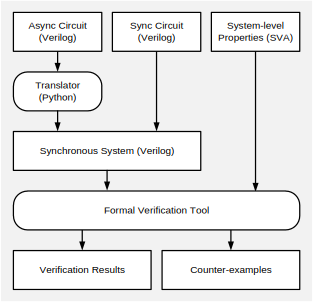
\includegraphics[width=8.8cm]{figures/fig_mixed_flow}

\caption{
Verification flow for a mixed sync-async system
}

\label{fig_mixed_flow}
\end{center}

\end{figure}


Our results from running this example were as follows. Both \ind{} and Xprova
proved that (1) no more than a~single CPU can access the bus simultaneously
and (2) the system does not enter a deadlock state, consistent with our
expectation. We modified the power management unit to introduce a fault and
allow all three CPUs to be active at the same time. This was discovered by
both tools -- both generated counter-example waveforms showing deadlock
occurrences.

% fig_system

\begin{figure}[!t]
\begin{center}

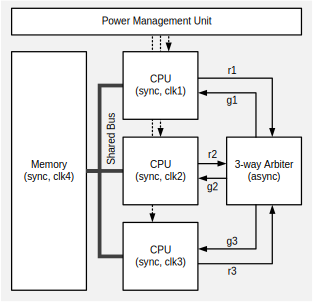
\includegraphics[width=8.8cm]{figures/fig_system}

\caption{
Use case example for mixed sync-async verification: a multi-clock domain system with an asynchronous arbiter.
}

\label{fig_system}
\end{center}

\end{figure}


% fig_arbiter

\begin{figure}[!t]
\begin{center}

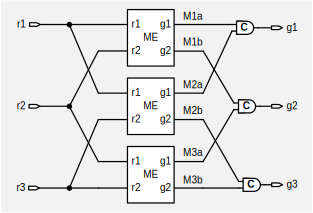
\includegraphics[height=6cm]{figures/fig_arbiter}

\caption{
Implementation of the 3-way arbiter in \Cref{fig_system}
}

\vspace{-0.6cm}

\label{fig_arbiter}
\end{center}

\end{figure}


This example demonstrates two points. First, we are able to perform
system-level verification of a mixed sync-async system using formal tools for
synchronous logic. Second, system-level verification can be used to prove or
disprove properties that cannot be verified at the component-level without
making unverified environmental assumptions. In our case, we proved that the
arbiter does not enter a deadlock state by verifying it against other modules
directly. If we verified the sync and async parts separately instead (as shown
in \Cref{fig_overview}A), we would need to create an accurate formal model of
the power management unit -- a very non-trivial task.
